% Evidence: Analysis 019 / 02_audit_runtime.py; observations/O002-runtime.md.
% Original implementation, qualification and compatibility: Runs 022, 025, 029.
\subsection{Realizing sparsity with specialized inference kernels}
\label{sec:kernel-autoresearch}

Released TwELL kernels accelerated their supported workload, but the unchanged
small-width primitive failed Pythia-14M qualification. Its adapted P0
descendant qualifies on only four of our 30 checkpoints; the $0.8910\times$
subset mean is not comparable to a full-cohort mean
(Appendix~\ref{app:kernel-results}). We use a human-guided coding-agent loop
and replay 42 eligible proposals against native PyTorch/SDPA CUDA graphs.
The workload is one RTX5090, BF16, batch one, uncached 2,048-token inference
with full vocabulary logits. Qualification checks logits and loss within
specified tolerances on all 338 validation blocks. The recorded agent default
is \emph{gpt-6-astra}; per-request served models and superiority over
human-only development are unverified.

\begin{figure}[!htbp]
\centering
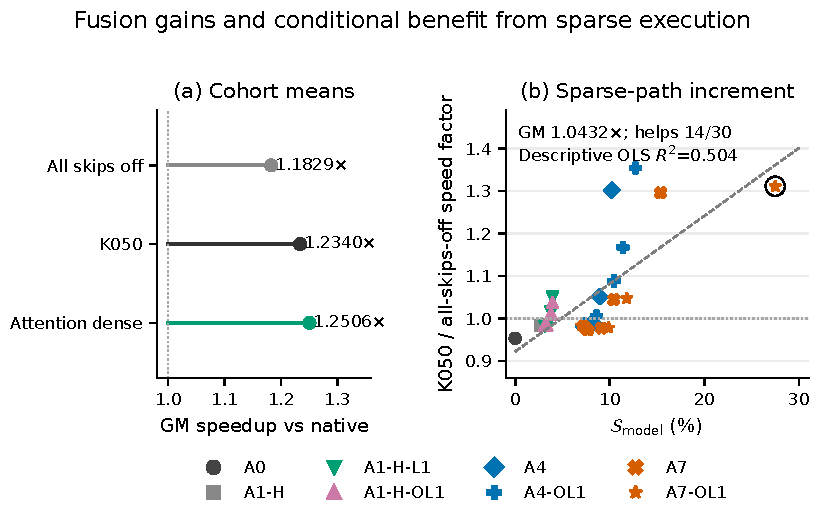
\includegraphics[width=\linewidth]{figures/07-kernel-attribution.pdf}
\caption{\textbf{Fusion gains and a conditional contribution from sparse execution.}
(a) Equal-checkpoint geometric mean native-relative speedups over all 30
14M checkpoints. (b) K050's speedup divided by all-skips-off's; values above
one favor sparse paths. The circle marks the search checkpoint; the dashed
line is descriptive OLS. Timings use the BF16 workload above, while the
horizontal axis uses canonical FP16 counts. Axes are restricted; neither the
fit nor same-checkpoint ratios establish a quality-matched model advantage.}
\label{fig:kernel-autoresearch}
\end{figure}

Selected K050 qualifies on all 30 checkpoints, with geometric mean
native-relative speedup $1.2340\times$. Its search retrospective reaches
$1.7830\times$ at the fixed A7-OL1, $\kappa=0.5$ checkpoint; Appendix~\ref{app:kernel-results}
retains the history and distinguishes the final-sweep maximum.
Fusion alone gives $1.1829\times$ (Figure~\ref{fig:kernel-autoresearch}).
Relative to that matched all-skips-off control, sparse paths add
$1.311\times$ at the search checkpoint and $1.043\times$ geometrically,
helping 14 of 30 checkpoints. These factors derive from separately measured
native-normalized timings. Their association with canonical FP16 sparsity
is weaker than native-relative speedup's ($R^2=0.5037$ versus $0.8167$);
Appendix~\ref{app:runtime-sensitivity} retains all descriptive sensitivity
checks and absolute latencies. BF16 timing and FP16 counts remain distinct.

Disabling attention skipping improves every checkpoint, raising the mean to
$1.2506\times$. The kernel skips an instruction when either complete operand
fragment is zero. It bypasses $58.0\%$ of eligible $QK$ and $67.2\%$ of
$PV$ instructions at the search checkpoint, yet runs slower than the dense
attention ablation. Partial zeros can still require an instruction, while
detection and control cost time. Scalar zero opportunity alone therefore
does not identify profitable execution.
